% THIS IS A LATEX TEMPLATE FILE FOR PAPERS INCLUDED IN THE
% *Anthology of Computers and the Humanities*. ADD THE OPTION
% `final' WHEN CREATING THE FINAL VERSION OF THE PAPER. 
% DO NOT change the documentclass
%\documentclass[final]{anthology-ch} % for the final version
\documentclass[final]{anthology-ch}         % for the submission

% LOAD LaTeX PACKAGES
\usepackage{booktabs}
\usepackage{graphicx}
\usepackage{multirow}
\usepackage{xcolor}
\usepackage{colortbl}
\usepackage{fancyvrb}
\usepackage{fbox}
\definecolor{teal}{RGB}{41, 115, 115}
\definecolor{salmon}{RGB}{255, 133, 82}
% ADD your own packages using \usepackage{}
\usepackage{adjustbox}
\usepackage{float}
\usepackage{tikz}
\usetikzlibrary{positioning, shadows.blur, arrows.meta}


\tikzset{
  stage/.style = {
    draw,
    rounded corners=2pt,
    minimum width=30mm,
    minimum height=11mm,
    inner sep=6pt,
    font=\rmfamily\footnotesize,
    top color=salmon!18,
    bottom color=salmon!8,
    blur shadow={shadow xshift=0.3ex,
      shadow yshift=-0.3ex,
      shadow blur steps=10,
      shadow blur extra rounding=0.5pt,
    }
  },
  arrow/.style = {
    -{Stealth[length=3.5pt, width=4pt]},
    very thick
  },
  label/.style = {
    font=\scriptsize\rmfamily,
    inner sep=0pt
  },
}

% TITLE OF THE SUBMISSION
% Change this to the name of your submission
\title{Reading Beyond the Center. Modeling Book Encounters in the Danish Periphery (1800-1850)}

% Literary Horizons Beyond the Center
% Modelling Book Spread 
% Modelling Book Offer
% Encountering Books

% AUTHOR AND AFFILIATION INFORMATION
% For each author, include a new call to the \author command, with
% the numbers in brackets indicating the associated affiliations 
% (next section) and ORCID-ID for each author. 

\author[1]{Alie Lassche}[
  orcid=0000-0002-7607-0174
]

\author[1]{Rie Eriksen}[
  orcid=0009-0002-1010-9627
]

\author[1]{Pascale Feldkamp}[
  orcid=0000-0002-2434-4268
]

\author[2]{Johan Heinsen}[
  orcid=0000-0001-9823-9009
]

\author[3]{Katrine Baunvig}[
  orcid=0000-0001-6706-6694
]

\author[1]{Kristoffer Nielbo}[
  orcid=0000-0002-5116-5070
]

% While we encourage including ORCID-IDs for all authors, you can
% include authors that do not have one by definining an empty ID.
%\author[2]{Pascale Feldkamp}[
%  orcid=
%]

% There should be one call to \affiliation for each affiliation of
% the authors. Multiple affiliations can be given to each author
% and an affiliation can be given to multiple authors. 
\affiliation{1}{Center for Humanities Computing, Aarhus University, Aarhus, Denmark}
\affiliation{2}{MASSHINE, Aalborg University, Aalborg, Denmark}
\affiliation{3}{Center for Grundtvig Studies, Aarhus University, Aarhus, Denmark}

% KEYWORDS
% Provide one or more keywords or key phrases seperated by commas
% using the following command
\keywords{historical newspapers, reading culture, periphery, book history, information extraction, GenAI}

% METADATA FOR THE PUBLICATION
% This will be filled in when the document is published; the values can
% be kept as their defaults when the file is submitted
\pubyear{2025}
\pubvolume{3}
\pagestart{78}
\pageend{101}
\conferencename{Computational Humanities Research 2025}
\conferenceeditors{Taylor Arnold, Margherita Fantoli, and Ruben Ros}
\doi{10.63744/YxKHrB4ZCThp}  
\paperorder{7}


\addbibresource{bibliography.bib}

%%%%%%%%%%%%%%%%%%%%%%%%%%%%%%%%%%%%%%%%%%%%%%%%%%%%%%%%%%%%%%%%%%%%%%%%%%%
% HERE IS THE START OF THE TEXT
\begin{document}

\maketitle

\begin{abstract}
This paper investigates the reading culture of peripheral regions in nineteenth-century Denmark by analyzing book advertisements in six local Danish newspapers, a source that provides valuable insights into the characteristics of literary culture and its mediation through the local press. Drawing on previous studies and theories of reading culture, book circuit, and cultural peripherality, this study challenges center-oriented narratives in studies of Danish reading culture. Using a pipeline that combines article classification, book title extraction with generative language models, and manual genre clustering, this paper presents a dataset comprising 900,000 digitized news articles, along with over 6,000 book titles extracted from newspaper advertisements. These titles are categorized into \textit{knowledge-} and \textit{leisure-oriented} reading, revealing a more diverse literary landscape than previously assumed. The data indicate coexisting practices of \textit{intensive} and \textit{extensive} reading and show significant variation across towns in both genre distribution and circulation patterns. The analysis reveals that each town in the periphery had its own distinctive reading profile, demonstrating that literary engagement in these regions was varied and locally rooted, rather than uniform or marginal.\footnote{To ensure reproducibility, code, embeddings, and raw data are available via \url{https://github.com/centre-for-humanities-computing/chr-book-ads}.}
\end{abstract}


\section{Introduction} 

The nineteenth century was a formative period in the development of Danish reading culture, as well as that of Europe more broadly \cite{st_clair_reading_2007}. As the publishing industry expanded and literacy became more widespread, the diversity of texts accessible to readers also increased. Traditionally, studies of nineteenth-century reading culture have primarily focused on the \textit{production} of literary works, and only in a limited sense paid attention to the \textit{spread} and \textit{reception} of books \cite{horstboll_menigmands_1999}. Moreover, when nineteenth-century Danish book culture has been addressed, it has often centered on urban, educated elites -- especially in relation to the literary movement of the Modern Breakthrough, which dominated cultural life in the late nineteenth century and was largely shaped by and for the cultural elite \cite{bjerring-hansen_deep_2023,bjerring-hansen_litteratursociologi_2023,hansen2024literary}.

That said, nineteenth-century reading culture was not limited to literary works alone, nor was the circulation of books confined to the upper segments of society. Although Copenhagen was already the largest city in Denmark, it had only approximately 130,000 citizens around 1850. The vast majority of Danes (around 80\% in 1840) lived in the countryside \cite{nielsen_daily_2014,christensen_danish_2006}. Most of them were farmers and agricultural servants. By studying their literary horizon, we expand our knowledge about the Danish book landscape, its diversity, nineteenth-century reading culture, as well as center/periphery dynamics in a historical information society.

In this paper, we explore the dissemination of books in peripheral regions of nineteenth-century Denmark, focusing on the literary horizon of communities geographically distant from major cultural centers (see \autoref{fig:map}). %and administrative centers.
These geographical areas have long and are still being viewed as marginal in relation to the urban and institutional core.\footnote{The terms \textit{Udkantsdanmark} (Peripheral Denmark) and \textit{den rådne banan} (the rotten banana) are still frequently used in political and public discourse in Denmark. The `rotten banana' refers to the outer regions of Denmark, which curve around the country in a banana-like shape. It reflects a perception that these rural areas are underdeveloped and place an excessive financial burden on society \cite{WINTHER,brodersen_den_2011}.} Because this segment of the population left behind few traceable records, we face significant gaps in traditional sources such as library holdings, lending registers, and other indicators of reading culture. To gain insight into reading culture in the periphery, we must turn to alternative sources. One such source are newspaper book advertisements -- often placed by booksellers \cite{appel_pa_2023} -- which have been shown to reflect local demand and circulation patterns \cite{darnton_what_1982}.

Book advertisements in newspapers only constitute one component of the commercial interface between booksellers and the readers, but their relative prominence must be understood in light of the specific conditions of early nineteenth-century Denmark, namely censorship and the Danish state bankrupty of 1813. Censorship imposed substantial restrictions on the circulation of printed material, thereby limiting the extent to which alternative media such as pamphlets or posters could be freely employed \cite{Høegh-Guldberg_Jensen_Danmarkshistorien}. Newspapers publishers, by contrast, often held licenses permitting them to advertise and were more resilient in financial terms \cite{Søllinge_Thomsen_Danske}. This contributed to making newspapers not only the most stable medium for commercial communication but also the most consistently expanding medium throughout the century \cite{horstboll_menigmands_1999}.

While book advertisements can thus not be assumed to reflect exactly what was read, they offer a valuable proxy for what was available, promoted, and likely to have circulated locally.\footnote{Provincial booksellers would either acquire books from bigger booksellers in Copenhagen and pay them back later or they would avoid debt by only buying books that they knew were on demand \cite{appel_pa_2023}.} As commercial texts responding to local demand and aimed at a broad regional public, they provide a more immediate and inclusive snapshot of reading culture -- particularly in areas underrepresented in formal archives, where lending libraries were scarce and state-library infrastructure limited \cite{horstboll_menigmands_1999}.\footnote{Note that lending libraries often were owned by the booksellers \cite{horstboll_menigmands_1999}.} Moreover, advertisements may capture demand across categories more evenly. Whereas lending library catalogues -- the most common source for book circulation -- tend to reflect a selective image of book culture skewed toward literary fiction, books for personal or devotional use, such as psalmbooks and religious texts, were more often purchased than borrowed \cite[345]{horstboll_menigmands_1999}.

We therefore study book advertisements in local newspapers to gain insights into the types of texts available and read, how reading culture was mediated through the local press, and how these peripheral regions were connected and related to one another in terms of reading culture. We seek to answer three simple questions about reading culture in the Danish periphery in this paper: \textit{what did people read}, \textit{how did people read}, and \textit{where did people read what}?

This paper is structured as follows: \autoref{sec:related_works} reviews related work on nineteenth-century reading culture and information extraction from historical texts. In \autoref{sec:data} we provide a description of the formation and content of the corpus used in this study. Our methodological pipeline is outlined in \autoref{sec:pipeline}, which includes the training of classifiers for article categories and book announcements, the extraction of book titles using generative language models, and the clustering procedure applied to the extracted book titles. In \autoref{sec:results}, we will answer the questions outlined above. In the final section, we present the conclusions and offer suggestions for future research.

\begin{figure}
  \centering
  \includegraphics[width=0.6\linewidth]{figures/map_dk.png}
  \caption{Map of Denmark with in dark green the towns whose newspapers are included in our corpus.}
  \label{fig:map}
\end{figure}

\section{Related Work}
\label{sec:related_works}

\subsection{Nineteenth-century reading culture}

The nineteenth century saw transformative changes in European book and reading culture, driven by technological advances, lower production costs, and socio-cultural shifts. In Denmark, improved printing technologies and the introduction of compulsory education in 1814 significantly widened access to printed materials, extending literacy beyond urban elites and into broader segments of the population, including rural communities \cite{Hertel,horstboll_menigmands_1999}. Scholarly debates about reading practices have traditionally highlighted a shift from \textit{intensive} reading (deep engagement with a limited selection of books) towards \textit{extensive} reading (covering a wider range of texts). This shift was described by \textcite{engelsing_perioden_1978} as the `reader revolution', driven by a rising bourgeois reading public in the late eighteenth and early nineteenth centuries. However, recent research suggests that this development was neither uniform nor immediate, particularly in rural or peripheral regions. Studies from the Netherlands, for instance, indicate that middle-class readers lacked literary socialization, often struggling to navigate a rapidly expanding literary market \cite{goedegebuure_lezersrevolutie_1993}. Similar dynamics can be assumed for rural Denmark, where existing research highlights a strong dominance of religious literature among rural readers \cite{jensen_vestjydsk_1943}.

Yet, despite these insights, detailed empirical evidence on reading practices in nineteenth-century Danish rural communities remains sparse. Existing studies largely employ qualitative methods and have predominantly focused on urban centers or earlier periods \cite{horstboll_menigmands_1999,appel_laesning_2001,appel_pa_2023,Ostling}. This creates significant gaps, especially regarding what rural populations actually read, how they accessed literature, and how reading habits evolved over time. Newspapers, alongside the novel, played a key role in addressing these gaps. As Benedict \textcite{anderson_imagined_2016} influentially argued, newspapers were instrumental in shaping national public spheres by simultaneously circulating information and cultural narratives to geographically dispersed readers, thereby fostering shared identities . By providing regular updates on books available to readers, newspaper book advertisements functioned as crucial mechanisms of literary dissemination, selection, and reader formation in peripheral regions.

In Denmark, newspapers significantly influenced the literary culture of peripheral areas by serving as a primary source of information about available literature. This influence was particularly important given the scarcity of public libraries or established literary institutions outside major urban centers. Consequently, examining newspaper book advertisements provides direct insight into how literary materials were marketed to, and perceived by, peripheral readers who may not yet have developed clear strategies for selecting literature -- thus offering a clearer picture of literary socialization processes outside elite urban circles. Moreover, in \textit{What is the History of Books?} \cite{darnton_what_1982}, Robert Darnton highlights the key role of booksellers in the circulation of literature. His example of Isaac-Pierre Rigaud, who ordered Voltaire’s \textit{Questions sur l’Encyclopédie} based on customer demand, illustrates how a bookseller’s stock can reflect a community’s literary interests.\footnote{How we study reading culture really depends, of course, on how we choose to define it -- and that remains an open, and surprisingly underdiscussed, question, both conceptually and methodologically. In peripheral and historical settings like this one, the challenge is sharper: sources are sparse, indirect, and often shaped by the institutions we are trying to look past. Book advertisements offer one possible proxy for reader interest and literary availability, while naturally capturing only one moment in the circulation process: the commercial interface between supply and anticipated demand. Other routes are possible: marginalia, lending records, letters, even oral accounts. But each method makes a different kind of reading visible -- and leaves others out.}

%A particularly instructive example of using print sources to explore reading culture among socially marginal groups is Charlotte Appel and Nina Christensen’s research on children's literature in Denmark (1750–1850) \cite{appel_laesning_2001}. Their study demonstrates how focusing on peripheral groups and neglected genres -- like children's books -- can significantly enrich our understanding of historical reading cultures and the broader literary landscape.

%By drawing on newspaper book advertisements from peripheral communities -- where middle and lower classes constituted the vast majority of the population -- we aim to similarly uncover more nuanced and representative patterns of literary consumption in nineteenth-century Denmark, moving beyond traditional narratives centered on urban elites.

In summary, we identify three main gaps in the existing literature. First, peripheral reading cultures remain underexamined in quantitative research. While recent book history has adopted computational methods, these have primarily focused on urban or institutional contexts, often overlooking rural regions and reading as a daily, non-prestigious activity. Second, empirical evidence on nineteenth-century Danish reading practices is scarce. Aside from case studies, there is little systematic knowledge of the types of books that were read or made available outside Denmark’s urban centers -- or of how reading habits evolved, for instance, from intensive to more extensive modes of reading. Third, the mechanisms of book dissemination remain understudied concerning reader formation. Despite Darnton’s call to attend to intermediaries like booksellers, little attention has been paid to how book advertisements functioned as selective interfaces between supply and demand, and in curating literary socialisation -- particularly in regions with weak literary infrastructure. By directing our attention to peripheral communities -- where the middle and lower classes made up 97\% of the population in 1801 and 1834 \cite{JohansenHansChr2021} -- and using newspaper book advertisements as a proxy for literary availability and interest, we are better positioned to examine reading culture beyond the cultural elite.


\subsection{Information extraction from historical texts}

Extracting information from historical texts is challenging due to factors like spelling variation, OCR errors, and the complexity of low-resource languages such as Danish. While Named Entity Recognition (NER) is commonly used for structured data extraction in historical sources \cite{Kettunen2016,kettunen_detecting_2019,pettersson_swener-1800_2024}, it is not well-suited to the task of identifying book titles, which are highly variable, context-dependent, and often embedded in noisy advertisement layouts. Previous work has shown that even combining manual and automated methods for detecting book-related content remains a complex, interpretive task \cite{samuelsson_between_2025}.

The emergence of generative language models (GenAI) has opened new possibilities for extracting information from historical corpora \cite{karjus_machine-assisted_2024}, though performance still varies by domain and task \cite{dalfsen2024direct, borst_death_2023, tudor_prompting_2025}. For this study, we developed a tailored approach that combines LLM-based extraction with human validation, specifically designed for the structure and ambiguity of nineteenth-century Danish book advertisements.


\section{Data}
\label{sec:data}

Our dataset comprises digitized articles from six nineteenth-century Danish local newspapers, which were selected based on their distribution in peripheral regions of Denmark. This includes newspapers from the towns of Aalborg, Aarhus, Maribo, Odense, Thisted, and Viborg (see \autoref{fig:map}). All newspapers are digitally available %via Mediestream, 
at the Danish Royal Library’s online platform.\footnote{\url{https://www.mediestream.dk}.} Although OCR-processed, the digitized texts exhibit a high word-level error rate, generally around 50\%. This is due to deterioration, small print, and cheap paper, but also cost-cutting decisions made by the Danish Royal Library to digitize from existing microfilm copies. Faulty column identification is another issue. % %A line of recent 'manual' distant readings utilize this material% For purposes like the one of this paper, this output is unusable. 
%Such frustrations have led to the 
A re-digitization initiative has been led by the ENO project \cite{heinsen_world_2025},\footnote{Hosted by \textit{Masshine} and \textit{The Historical Data Lab} at Aalborg University: \url{https://hislab.quarto.pub/eno/}.} which involves re-OCRing the newspapers using models developed in Transkribus \cite{kahle_transkribus_2017}, a tool originally designed for Handwritten Text Recognition (HTR). The word-level error rates are typically less than 5\% for the re-OCRed data, and the column segmentation is near faultless. ENO is an ongoing project, beginning with the oldest newspapers and progressing forward.\footnote{The most recent version of the ENO-corpus is available on \url{https://huggingface.co/datasets/JohanHeinsen/ENO}.} The current study utilizes reprocessed newspapers from the first half of the nineteenth century, when newspapers had become widely available across Denmark. While they do not all cover the same period, the overlapping time span across all titles is from 1824 to 1838.\footnote{The version of the corpus used in this paper, is available on \url{https://huggingface.co/datasets/chcaa/chr-book-ads-articles}.} The size of each newspaper dataset differs, reflecting the frequency with which the newspapers appeared at the time. Refer to \autoref{tab:stats_corpus} for statistics on the corpus.

\begin{table}[h]
\small
  \centering 
  \begin{tabular}{lrccrrr}
    \toprule
    \textbf{Newspaper} & \textbf{Population} & \textbf{Period} & \textbf{Frequency/week} & \textbf{Editions} &\textbf{Articles} & \textbf{Words} \\
    \midrule
    Aalborg & 6,500 & 1818-1842 & 3-5 & 5,075 & 156,011 & 19,872,861 \\
    Aarhus & 6,000 & 1794-1845 & 2-4 & 8,288 & 258,414 & 28,130,531 \\
    Maribo & 1,000 & 1809-1838 & 2-3 & 2,990 & 85,092 & 7,845,803  \\
    Odense & 8,000 & 1809-1848 & 4-6 & 8,240 & 202,178 & 31,558,778 \\
    Thisted & 1,600 & 1824-1848 & 1-3 & 3,238 & 72,102 & 9,468,784 \\
    Viborg & 3,100 & 1809-1842 & 2-4 & 5,161 & 169,638 & 17,421,450 \\
    \midrule
    \textit{Total} & & &  & 32,992 & 943,435 & 114,298,207 \\
    \bottomrule
  \end{tabular}
  \caption{Descriptive statistics on the corpus and subcorpora. The \textit{population} is expressed in the number of inhabitants of that town, taken from the average of inhabitants in 1801 and 1845. These years were selected because they correspond with national census data collection periods in Denmark. The \textit{frequency} column describes the number of times a newspaper appeared per week. The number of editions refers to the number of unique newspapers from that town in our dataset.}
  \label{tab:stats_corpus}
\end{table}

As part of the ENO-initiative, the raw output from Transkribus has been post-processed through a pipeline that combines rule-based components with modeling based on structural features at the line level. Features include elements such as line length, punctuation, and hyphenation. The aim is for each newspaper edition to be segmented into its individual articles. The complexity of this task varies across newspapers and is heavily dependent on their layout. %This is also a work in progress, and the segmentation is far from perfect. 
The segmentation process is ongoing and still imperfect, with common errors including the merging of unrelated text segments or the splitting of single articles into smaller fragments -- both of which complicate downstream categorization using LLMs.

\section{Methods}
\label{sec:pipeline}
\autoref{fig:pipeline} shows the four-step pipeline used to extract and cluster book titles. The subsequent sections provide a detailed description of each step.

\begin{figure}[H]
  \centering
  \begin{adjustbox}{width=\linewidth}
  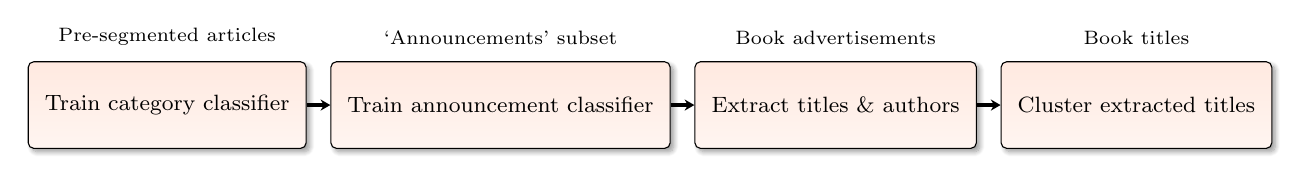
\begin{tikzpicture}[node distance=32mm and 3mm]
    \node[stage] (cat)      {Train category classifier};
    \node[stage, right=of cat]          (ann)  {Train announcement classifier};
    \node[stage, right=of ann]          (ext)  {Extract titles \& authors};
    \node[stage, right=of ext]          (clu)  {Cluster extracted titles};
    \draw[arrow] (cat) -- (ann);
    \draw[arrow] (ann) -- (ext);
    \draw[arrow] (ext) -- (clu);
    \node[label, above=2mm of cat] {Pre-segmented articles};
    \node[label, above=2mm of ann] {`Announcements' subset};
    \node[label, above=2mm of ext] {Book advertisements};
    \node[label, above=2mm of clu] {Book titles};
  \end{tikzpicture}
    \end{adjustbox}
  \caption{Four-stage pipeline for title extraction and clustering.}
  \label{fig:pipeline}
\end{figure}


\subsection{Training classifier for article categories}

In the steps taken to post-process the articles, a separate set of rules was applied to assign a category to each article: National News (\textit{Indenlandsk/Fædrelandet}), International News (\textit{Udenlandsk/Blandet}), Announcements (\textit{Bekjendtgjørelser}), and a small section for Reader Mail (\textit{Indsendt}). The accuracy of this categorization step varies by newspaper and depends largely on layout structure. Manual inspection confirmed that the Maribo newspaper achieved accurate segmentation and categorization, owing to its particularly clear and consistent layout. To evaluate the performance of different text representations for article classification, we used a balanced sample (24,000 articles for each category) of pre-categorized articles from the Maribo newspaper as a testing ground. We experimented with two types of representations: TF-IDF and semantic embeddings generated using the \texttt{multilingual-e5-large} model.\footnote{\url{https://huggingface.co/intfloat/multilingual-e5-large}. Note that the articles were divided into chunks of the maximum length supported by the model (514). Each segment was individually embedded, and the mean of these embeddings was used to represent the article as a whole. The embeddings of the articles used in this study are available on \url{https://huggingface.co/datasets/chcaa/periphery-aviser-e5}.} Because the \textit{Indsendt} category was frequently misclassified as \textit{Indenlandsk}, we chose to merge it into the latter category, seeing that our main goal was to label the `Announcements' correctly. Proceeding with a three-class classification task, we trained and evaluated a Logistic Regression model using a 70/30 train-test split.\footnote{We used the \texttt{scikit-learn} package in Python \cite{pedregosa_scikit-learn_2011}.} Both representations yielded similar results, with F1-scores for individual classes ranging between 0.84 and 0.95.

The trained model was then used to predict the category of an unseen set of 1,000 articles, taken from the remaining newspapers. We manually evaluated the predicted category for each article -- creating a balanced gold standard -- and calculated the classification accuracy for both feature types. Since the semantic embeddings slightly outperformed the TF-IDF features (with accuracies of 0.91 vs. 0.89), we used semantic embeddings in the subsequent classification.
For the final classification model, we expanded the gold standard with a random sample of 200 additional articles from the correctly-segmented Maribo newspaper, ending up with a gold standard in which all newspapers were equally represented. The model trained on this benchmark dataset, whose performance metrics are included in \autoref{tab:classification_results_categories}, was then used to predict the category of the remaining unlabeled articles, resulting in the distributions shown in \autoref{fig:words_month_category}.

\begin{table}[h]
\small
\centering
\begin{tabular}{lccc}
\toprule
\textbf{Class} & \textbf{Precision} & \textbf{Recall} & \textbf{F1-score} \\
\midrule
Announcements & 0.88 & 0.82 & 0.85 \\
National news       & 0.72 & 0.82 & 0.77 \\
International news        & 0.89 & 0.82 & 0.85 \\
\bottomrule
\end{tabular}
\caption{Performances of the classification task to label newspaper articles by category.}
\label{tab:classification_results_categories}
\end{table}

\begin{figure}
  \centering
  \includegraphics[width=0.8\linewidth]{figures/words_month_category.png}
  \caption{Number of words per month for the six newspapers in our corpus. The colors correspond with the type of article.}
  \label{fig:words_month_category}
\end{figure}

\subsection{Training classifier for book announcements}

We created a gold standard sample from the Announcements category, consisting of articles that mention book titles. This involved manually evaluating articles that contained search terms we had previously identified as indicators of book announcements.\footnote{We used the following search terms: `indb.', `heftet', `udkomm', `udgiv', `udgav', `indbund', `oversatt', and `paa adressekontoiret'. We acknowledge that this list introduces a potential bias in the gold standard, as it may exclude book advertisements that do not contain these terms. However, due to the highly formulaic and programmatic nature of advertisement phrasing in these newspapers, we expect this approach to capture the vast majority of book-related announcements.} From the manually assessed articles, we selected a balanced sample of 540 -- half book announcements and half non-book announcements -- to train a Logistic Regression model. The model was evaluated using fivefold cross-validation, with semantic embeddings serving as input features. Performance metrics are presented in \autoref{tab:classification_results_books}. We then applied the model trained on the fifth fold to the remaining articles in the Announcements category, identifying 7,531 likely book announcements.\footnote{Before making predictions for the remaining articles in the Announcement category, we filtered out announcements that appeared five times or more in the dataset, since manual inspection showed that these were never book announcements. We also filtered out all announcements that reported on lottery drawings, as well as announcements shorter than 70 characters and longer than 500 characters.}

\begin{table}[h]
\small
\centering
\begin{tabular}{lccc}
\toprule
\textbf{Class} & \textbf{Precision} & \textbf{Recall} & \textbf{F1-score} \\
\midrule
Book announcement & 0.91 & 0.92 & 0.91 \\
Non-book announcement       & 0.92 & 0.90 & 0.91 \\
\bottomrule
\end{tabular}
\caption{Performances of the classification task to label book announcements.}
\label{tab:classification_results_books}
\end{table}

\subsection{Extracting book titles}

To extract book titles and authors from the classified book announcements, we employed a generative language model via the OpenAI API. Specifically, we used the \texttt{gpt-4o-mini} model, configured with $temperature=0.3$ and $max\_tokens=800$. For each article, we supplied the full text of the announcement and prompted the model to return a list of mentioned book titles and their authors, along with an English translation of each title. We experimented with several prompt formulations to determine which would yield the most accurate extractions. To evaluate the adequacy of each prompt, we used a manually annotated gold standard of 300 book announcements. This sample was randomly created and curated by two human annotators.\footnote{These were a graduate student in religious studies and a postdoctoral researcher in history, both with literary backgrounds and expert knowledge of historical newspaper material.} For every book announcement, annotators extracted the book titles, authors, and the English translation of the title. An example illustrating the structure of this annotated sample is presented in \autoref{tab:gold_standard_books}. When a book announcement did not contain a book title, we filled in `NO\_BOOK' in every column.

\begin{table}[h]
\small
\centering
\begin{tabular}{llll}
\toprule
\textbf{article\_id} & \textbf{original\_title} & \textbf{translated\_title} & \textbf{author} \\
\midrule
aal\_007242 & Jliade & Iliad & Homer \\
aal\_028045       & Bibelen forsvarer sig selv & The Bible defends itself & Biskop Balle \\
ode\_193405 & Kjerlighedens Gierninger & The Works of Love & S. Kierkegaard \\
\bottomrule
\end{tabular}
\caption{Example of the curated set of gold standard book announcements.}
\label{tab:gold_standard_books}
\end{table}

Extraction quality of the various prompts was assessed using fuzzy matching on the gold standard set. For each model output, we required an exact match on the \texttt{article\_id}, and a partial match on either only the \texttt{original\_title} or both the \texttt{original\_title} and the \texttt{author}. We used the \texttt{fuzz} function in the \texttt{rapidfuzz} package and experimented with thresholds ranging from 65 to 80.

In addition to the three prompts we manually designed, we also leveraged the self-improving capabilities of generative language models by implementing a feedback loop \cite{yu_sipdo_2025}. After generating outputs for a subset of book announcements using an initial prompt, we provided the model with ten of its true positives and ten of its false positives. We then asked the model to reflect on discrepancies and suggest improvements to the prompt formulation itself. This process allowed the model to iteratively refine its own instructions based on its performance, enabling us to test whether prompt optimization through in-context feedback could yield higher extraction accuracy. We compared prompts (P) based on their precision, recall, and F1-score, which are included in \autoref{tab:title_extraction_results} in \autoref{appdx:prompt_perform}. P1, P2, and P3 are the prompts that were manually created, while P4, P5, P6, and P7 were created in the feedback loop of the generative model.\footnote{All prompts are included in \autoref{appdx:prompts}.} While the performances of P4 and P5 were considerably lower than that of our own prompts, they were matched and slightly outperformed by P6 and P7.

The prompt that yielded the best results struck the right balance between providing enough guidelines without overcomplicating the task. This prompt (P6 in \autoref{appdx:prompts}) was used for extracting titles from all predicted book announcements, resulting in 6,391 extracted titles. \autoref{tab:stats_announcements} contains more detailed statistics on the extracted titles.

\begin{table}[h]
\small
  \centering 
  \begin{tabular}{lccr}
    \toprule
    \textbf{Newspaper}  & \textbf{Announcements} & \textbf{Book announcements} & \textbf{Titles} \\
    \midrule
    Aalborg  & 62,615 (40\%) & 560 (0.9\%) & 965 \\
    Aarhus  & 113,783 (44\%) & 848 (0.7\%) & 1,313 \\
    Maribo  & 35,817 (42\%) & 629 (1.8\%) & 1,049  \\
    Odense  & 82,999 (41\%) & 890 (1.1\%) & 1,568  \\
    Thisted  & 15,006 (20\%) & 222 (1.5\%) & 642 \\
    Viborg  & 61,635 (36\%) & 556 (0.9\%) & 854 \\
    \midrule
    \textit{Total} & 371,855 & 3,705 & 6,391 \\
    \bottomrule
  \end{tabular}
  \caption{Number of articles, announcements, and book titles after extraction.}
  \label{tab:stats_announcements}
\end{table}

\subsection{Clustering extracted book titles}
After post-processing the extracted titles, all entries were manually assigned to semantic categories by the same two annotators, along with two student assistants with backgrounds in literary studies. The categories were derived from the corpus itself: through repeated close reading and annotation, the annotators identified recurring themes and patterns in the titles. Based on internal discussions, this resulted in the following categories: \textit{Agriculture, household and artisanship}; \textit{Almanacs and other light readings}; \textit{Education and Bildung}; \textit{Geography, topography and biology}; \textit{History, philosophy and biographies}; \textit{Law, politics and government}; \textit{Literature and personal writings}; \textit{Religion, theology and psalms}; \textit{Subscription journals}; \textit{Theatre, music and poems}; and \textit{Unknown}.\footnote{The \textit{Unknown} category includes books for which no additional information could be found online, and whose titles provided no clear indication of their topic or theme. These were mostly anonymous works with very short, generic titles.}

\section{Results}
\label{sec:results}

\begin{figure}
  \centering
  \includegraphics[width=\linewidth]{figures/cat_sizes.png}
  \caption{Number of book titles in each manually assigned category in the corpus.}
  \label{fig:cat_sizes}
\end{figure}

\subsection{Knowledge- and leisure-oriented reading} % what did they read?
The horizontal bars in \autoref{fig:cat_sizes} show the distribution of the 6,391 book titles across the manually assigned categories. Upon closer inspection, the ten substantive categories (excluding \textit{Unknown}) fall into two broader thematic clusters.
The first comprises texts oriented toward knowledge acquisition, instruction, or moral and civic education. This includes, first and foremost, the categories \textit{Education and Bildung} (largely schoolbooks) and \textit{Agriculture, household and artisanship} (practical manuals for work in and around the rural household), as well as the categories \textit{Law, politics and government}, \textit{Geography, topography and biology} and \textit{Religion, theology and psalms}, the latter primarily concerned with spiritual development. We can summarize these texts as `knowledge-oriented reading'. The second cluster comprises texts related to leisure, cultural consumption, and personal enjoyment. This encompasses the categories \textit{Theatre, music and poems}, \textit{Literature and personal writings}, \textit{Almanacs and other light readings}, and \textit{History, philosophy and biographies}. These fall under what we call `leisure-oriented reading'. 

Among the 6,391 book titles we extracted, we distinguished 4,141 unique book titles.\footnote{These are unique combinations of author and book title.} Of these, 3,171 appear only once in the dataset. The remaining 970 book titles are advertised between 2 and 55 times. The 20 titles that appear most frequently in advertisements are listed in \autoref{tab:books} in \autoref{appdx:top20_authors_books}. Most of these fall into the cluster of `knowledge-oriented reading', including several religious handbooks and psalmbooks, handbooks for reading and mental arithmetic, and a recipe book. In terms of authorship, the dataset contains 1,706 unique names -- 1,049 appear only once, while the remaining 657 authors are mentioned between 2 and 144 times. The 20 most frequently advertised authors are listed in \autoref{tab:authors} in \autoref{appdx:top20_authors_books}. This list includes figures associated with `knowledge-oriented reading' -- such as A. F. Just, N. Blicher, and C. Jacobsen -- as well as prominent literary authors tied to `leisure-oriented reading', including Adam Oehlenschläger, August von Kotzebue, Walter Scott, Ludvig Holberg, and H. C. Andersen.

Together, these categories and clusters reveal that the reading culture in nineteenth-century peripheral Denmark was far more diverse than previously assumed. While \textit{Religion, theology and psalms} -- the category most expected based on previous studies \cite{jensen_vestjydsk_1943} -- does appear in the top three with its 811 titles, it accounts for less than 13\% of the overall corpus. Notably, the category \textit{Theatre, music and poems} is even more prominent, with 1,310 titles -- 1.5 times as many. Moreover, we observe that `leisure-oriented reading' encompasses both high-culture and popular texts. Next to titles of the above mentioned well-known literary authors, the corpus also contains a substantial number of almanacs. Particularly noteworthy are the frequently occurring German `Taschenbücher'. These small, portable pocketbooks were designed for convenient reading and typically featured novellas, essays, and (often romantic) short stories, in addition to the poetry and calendar content characteristic of almanacs more generally. Several of them specifically targeted the female reader, being titled `Frauentaschenbuch' \cite{stegemeier_frauentaschenbuch_1937}. In addition to these popular publications, the dataset includes more than 300 German titles, suggesting that readers in the Danish periphery also read works in German alongside Danish literature.

\subsection{Intensive and extensive reading} % how did they read?

To get more insight into the longevity of a book title, we examine its advertising span -- that is, the time between the first and last time a book title appears in an advertisement within our corpus. Across all categories, most titles appear in advertisements for only one day. \autoref{tab:one_day} contains the percentages of books per category that have only been advertised for one day, and it shows they vary between 66\% (\textit{Religion, theology and psalms}) and 93\% (\textit{Unknown}). In the box plots in \autoref{fig:boxplots_books}, we show the distribution of the books that have been advertised for more than one day.

\begin{table}[h]
\small
\centering
\begin{tabular}{lr}
\toprule
\textbf{Category} & \textbf{Percentage} \\
\midrule
Agriculture, household and artisanship  &   69.5\% \\
Almanacs and other light readings      &   69.3\% \\
Education and Bildung                  &   72.5\% \\
Geography, topography and biology      &   75.9\% \\
History, philosophy and biographies    &   82.7\% \\
Law, politics and government           &   75.9\% \\
Literature and personal writings       &   76.6\% \\
Religion, theology and psalms          &   66.4\% \\
Subscription journals                  &   66.7\%\\
Theatre, music and poems               &   70.4\% \\
Unknown                                &   93.1\% \\
\bottomrule
\end{tabular}
\caption{Percentage of books per category that have an advertising span of one day.}
\label{tab:one_day}
\end{table}

The varying lengths of the boxes in \autoref{fig:boxplots_books} reflect notable differences in sustained visibility across categories. Titles in the categories \textit{Religion, theology and psalms} and \textit{Education and Bildung} tend to have markedly longer advertising spans, ranging from 16 to 38 years. This suggests persistent availability and enduring demand, likely tied to the long-term relevance and repeated use of these works. Such patterns resonate with what Engelsing has described as the \textit{intensive} reading practice -- the repeated engagement with a limited set of texts -- which he argued had largely been replaced by extensive reading by the end of the eighteenth century \cite{engelsing_perioden_1978}. Our findings nuance that claim, indicating that intensive reading practices, particularly in religious contexts, remained significant in nineteenth-century Denmark.

By contrast, categories like \textit{Literature and personal writings}, \textit{History, philosophy and biographies}, and \textit{Geography, topography and biology} display shorter advertising spans, suggesting a quicker turnover and greater influx of new titles. These categories appear more closely associated with an \textit{extensive} reading practice, characterized by broad, fast-paced consumption. This pattern likely reflects not only the content and intended use of the books -- often topical, narrative-driven, or single-read publications -- but also the commercial strategies of booksellers responding to fluctuating demand. While the longer lifespan of religious and educational titles signals stability and long-term relevance, the brevity in these other categories points to a more dynamic and diversified literary market.

\begin{figure}
    \centering
    \includegraphics[width=\linewidth]{figures/boxplot_lifespan_books.png}
    \caption{Advertising span of books that appear in advertisments over multiple days, grouped per category.}
    \label{fig:boxplots_books}
\end{figure}

\subsection{Unpacking the periphery} % where did they read what?

\begin{figure}
  \centering
  \includegraphics[width=\linewidth]{figures/norm_cats_newspapers.png}
  \caption{Normalized category distribution per newspaper.}
  \label{fig:norm_cats_newspapers}
\end{figure}

To assess whether town size is associated with the relative number of book announcements, we fitted a mixed-effects model with the $log$ of population size as a fixed effect and year as a random effect.\footnote{We used the \texttt{statsmodels} package in Python \cite{seabold2010statsmodels}.} The results show a statistically significant negative relationship between population size and the normalized count of advertised book titles ($\beta =-0.013, SE=0.001, z=-9.91, p<0.001$).\footnote{The number of book titles in a newspaper are normalized against the total number of editions of that newspaper.} This means that smaller towns, such as Maribo and Thisted, tended to have proportionally more book advertisements in their newspapers than larger towns.

To compare how the book title offerings differ across newspapers, we visualized the normalized distribution of categories for each newspaper in \autoref{fig:norm_cats_newspapers}.\footnote{The number of book titles per category are normalized against the total number of book titles advertised in that newspaper.} The stacked bar plots show that all categories are represented in each of the newspapers. Most visually dominant across all newspapers is the \textit{Theatre, music and poems} category. This category seems to occupy roughly one-fourth to one-third of the total content of the newspapers, confirming that cultural content had a more central role in local newspapers than previously anticipated. Especially Aalborg and Aarhus -- both towns with established theatres -- have a higher distribution of this category, likely reflecting a large readership with access to or interest in theatrical and artistic life. 

In contrast, towns such as Viborg, Maribo, and Odense show a relatively lower proportion of cultural content in this category -- although Odense, the largest town in our dataset, also had a theatre. This may suggest that interest in theatre does not necessarily correlate with population size, but rather reflects the composition of a population -- explaining why Aalborg and Aarhus, which are similar in geography and demographics, show comparable patterns. Instead, the newspapers in Viborg, Maribo, and Odense seem to emphasize the `knowledge-oriented reading', with a stronger presence of, for example, the category \textit{Religion, theology and psalms}. When we model the relationship between the shares of the categories \textit{Religion, theology and psalms} and \textit{Theatre, music and poems} in a mixed-effects model with year as random effect, we find that an increase in the \textit{theatre} share is associated with a decrease in \textit{religion} share ($\beta=-0.184, SE=0.058, z=-3.19, p=0.001$). This suggests that religious content in book advertisements is competing with the more cultural and artistic genres, often including profane music, satire, and critique of society. As seen in \autoref{fig:norm_cats_newspapers}, Viborg, in particular, stands out for this inverse relationship. This pattern aligns with the town's long-standing status as an important religious center in Denmark, exemplified by its cathedral, which dates back to 1065.

Overall, the newspapers of Aalborg and Aarhus show similar profiles, with balanced distributions across most categories. This is confirmed by the heatmap in \autoref{fig:heatmap}, which shows the cosine distances between the category distributions of each newspaper -- where each newspaper vector expresses the normalized counts per category: Aalborg and Aarhus exhibit the highest cosine similarity. Both towns were harbor cities with comparable population sizes (approximately 6,000-6,500 inhabitants) and were located relatively close to one another. It is therefore likely that their newspapers served similar audiences, which may explain the overlap in the advertised book offerings. The heatmap furthermore shows that the newspaper of Maribo -- located on the island Lolland-Falster -- has the largest cosine distance to the other newspapers, with its difference from the newspaper of Odense being the greatest. %Overall, the low distance values support the interpretation suggested by the stacked bar plots: the book titles offered are broadly similar across newspapers.

\begin{figure}
  \centering
  \includegraphics[width=0.5\linewidth]{figures/heatmap_cosine.png}
  \caption{Heatmap showing the cosine distances between category distributions in newspapers. The lighter color corresponds with a lower cosine distance, in other words, a higher similarity between two distributions. Note that we would expect cosine similarity values to be naturally high when comparing vectors this short (here, 11-category distributions). Rather than measuring overall similarity, the measure helps us focus on relative differences -- highlighting newspapers whose category distribution stands apart.}
  \label{fig:heatmap}
\end{figure}

Another notable observation is that the two smallest towns in the dataset, Maribo (700-1,400 inhabitants) and Thisted (1,100-2,100 inhabitants), exhibit a comparatively higher share of the category \textit{Education and Bildung} than the other newspapers. This pattern is visible in \autoref{fig:norm_cats_newspapers}, and is statistically supported by a mixed-effects model. When modeling the relationship between a town's population size and the normalized share of the \textit{Education and Bildung} category (with year as a random effect), we observe a significant negative association with population size ($\beta=-0.026, SE=0.006, z=-4.62, p<0.001$). This suggests that smaller towns tend to have a higher proportion of advertisements related to education compared to larger towns. One possible explanation lies in the social and institutional impact of the Danish School Acts of 1814, which made primary education compulsory across Denmark. While the legislation applied nationally, its practical implementation often had a greater visible effect in rural or less urbanized areas, where formal schooling structures were less developed beforehand \cite{Larsen2008}. In smaller towns, the new educational infrastructure -- such as the construction of schools, training of teachers, and dissemination of textbooks -- represented a significant cultural shift, generating increased demand for educational materials. The prominence of the \textit{Education and Bildung} category in newspapers from small towns like Maribo and Thisted may therefore reflect the intensity with which these reforms were being realized in those settings.

\section{Discussion and conclusion}
The analysis of nineteenth-century book advertisements in local newspapers from the Danish periphery has shed new light on an underexplored aspect of nineteenth-century reading culture. By applying classification models to categorize book advertisements and using a generative language model to extract book titles from them, we constructed a dataset of almost 6,400 book titles, comprising over 4,000 unique titles. With this dataset, we addressed three key questions about reading culture in peripheral Denmark: \textit{what did people read}, \textit{how did people read}, and \textit{where did people read what?} The findings show that the book offers in the advertisements both include texts associated with `knowledge-oriented' reading and `leisure-oriented' reading. This challenges earlier claims that nineteenth-century middle-class readers primarily consumed religious books. Instead, we observe a much more diverse reading landscape -- spanning genres, themes, and even languages -- than previously assumed.

In terms of reading practices, an analysis of advertising spans of book titles revealed evidence for both the \textit{intensive} and \textit{extensive} reading practice -- the former characteristic for books in the categories \textit{Religion, theology and psalms} and \textit{Education and Bildung}, the latter for books in categories such as \textit{Literature and personal writings} and \textit{History, philosophy and biographies}. This adds nuance to Engelsing's theory that extensive reading had replaced intensive reading by the beginning of the nineteenth century.

The newspaper-level analysis yielded further insights. We identified a statistically reliable negative relationship between the population size of a town and the proportion of book titles in its newspaper, indicating that smaller towns included more book titles in their newspaper advertisements. We also observed that religious content in book advertisements competes with the more cultural and artistic genres, with some newspapers leaning more strongly towards one or the other. Finally, we found that smaller towns tend to advertise more schoolbooks than larger towns, a pattern likely connected to the institutionalization of compulsory education in Denmark in 1814, which had a pronounced impact in rural and less urbanized areas. In summary, the study demonstrates that studying book advertisements in local Danish newspapers is a fruitful way to show that reading culture in the nineteenth-century Danish periphery was more varied and dynamic than earlier accounts have suggested.

Nevertheless, while advertisements reflect commercial strategies aimed at attracting readers, they should not be interpreted as direct measures of reader demand or popularity. The decision to advertise likely varies by genre. For some genres -- such as religious literature -- a lower advertising frequency may reflect stable, widespread circulation that made further promotion unnecessary. In contrast, genres with high advertising intensity may signal novelty, uneven distribution, or a bookseller’s expectation of future demand, rather than confirmed popularity. As \textcite{harris_remembering_1980} note, advertising often operates in tension with what is already assumed to be known by the audience, rather than simply mirroring public interest \cite{baunvig_fictional_2021}. Thus, continued advertising can suggest either actual sales success or an effort to create visibility for unfamiliar or aspirational content.\footnote{Since booksellers were often indebted to bigger Copenhagen-based booksellers, it seems unlikely that repeated advertisements indicate a book’s lack of popularity. Rather than signaling unsold stock, re-advertising likely reflects ongoing expectations of demand.}

Another limitation of the corpus and methods used in this study deserves mention. First, the segmentation of newspapers into individual articles is not always accurate, which may have affected the identification of book announcements -- some of which were incorrectly merged with unrelated content. We experimented with training a classification model to detect such cases, but these proved difficult to reliably identify. As a result, we limited the analysis to correctly segmented announcements. This likely means that the number of detected book advertisements underrepresents the actual total, though we assume this bias is consistent across newspapers and does not substantially affect comparative findings.

Interestingly, since the start of this study, significant improvements have been made in article segmentation methods for these historical newspapers. This gives us reason to be optimistic that future iterations of this study will benefit from more accurate segmentation, thereby enhancing both the completeness and reliability of the dataset. Additionally, more local newspapers are currently being digitized -- both to extend the chronological range of the corpus and to include a broader selection of titles. These developments will help make future studies based on this corpus more representative of the diversity and evolution of reading culture in the Danish periphery.

Our study opens up new possibilities for further research into nineteenth-century Danish reading culture. Two findings, in particular, warrant deeper investigation: the role of German-language books in Danish reading culture and the impact of the Danish School Acts on the availability and circulation of books in the periphery. At the same time, our approach speaks to broader questions of historical information dynamics in Denmark. The corpus and methods developed here could be applied to trace the dissemination of both national and international news, and to explore how local and regional reading publics were interconnected through the press. Extending the dataset to include Copenhagen-based newspapers would further enhance comparisons between center and periphery, allowing for a more comprehensive understanding of how information flowed within a historical information society. Beyond the Danish case, the pipeline presented in this study offers a scalable, adaptable framework for studying information circulation in other Western European contexts with similar media infrastructures -- contributing not only to the history of reading, but to the field of information history as a whole.


\section*{Acknowledgements}
The authors affiliated with Aarhus University were supported by grants from the Carlsberg Foundation (\textit{The Golden Array of Danish Cultural Heritage}) and the Aarhus Universitets Forskningsfond (\textit{Golden Imprints of Danish Cultural Heritage}). We would like to thank all participants of the ENO-team, as well as Kit Morgenstjerne and Ingeborg Reinholdt Thorhauge for their annotation work. Part of the computation done for this project was performed on the UCloud interactive HPC system, which is managed by the eScience Center at the University of Southern Denmark.





%This unnumbered section should be blank when submitting your paper. After review, you may include lists of people and organizations who supported the work.

% Print the biblography at the end. Keep this line after the main text of your paper, and before an appendix. 
\printbibliography

% You can include an appendix using the following command
\appendix

\section{Prompts} \label{appdx:prompts}

\footnotesize

\textbf{P1.} This is an announcement in a Danish nineteenth century newspaper. Extract the book titles and authors that are mentioned. Return results in this format:

original\_title: <title in Danish>

translated\_title: <title in English>

author: <author\_name> \\
If the author is missing or unclear, fill in `NO\_AUTHOR'. For the translated\_title, you can translate yourself. Be careful and look closely, sometimes the author name is a bit hidden. It can be that it is mentioned like this: `AUTHOR's TITLE is now available.' Look closely where the title begins and ends. When the announcement does not contain book titles, return exactly one row with:

original\_title: NO\_BOOK

translated\_title: NO\_BOOK

author: NO\_BOOK \\


\noindent \textbf{P2.} Here is an announcement in a Danish nineteenth century newspaper. If book titles and authors are mentioned, extract those in this format:

original\_title: <title in Danish>

translated\_title: <title in English>

author: <author name>\\
If the author is missing or unclear, fill in `NO\_AUTHOR'. The author name can appear in many ways, for example: `AUTHOR's TITLE is now available.' Look closely where the title begins and ends. For the translated title, translate it yourself in English. When the announcement does not contain book titles, return exactly one row with:

original\_title: NO\_BOOK

translated\_title: NO\_BOOK

author: NO\_BOOK\\
Here are first a few examples of announcements containing book titles: \\
Example1: "Baggesens allerældste Poesier."

`original\_title': allerældste Poesier; `author': Baggesen \\
Example2: "Kateketisk Magasin af J. C. Wegener, Forstander for det Kongelige Skolelærer-Seminarium paa Joenstrup." 

`original\_title': Kateketisk Magasin; `author': J.C. Wegener \\
Example3: "Ceres. Et periodisk Skrivt for dannede Læsere. Udgiver af F. M. Lange. Femte Hefte. Det indeholder: Juliette, eller det hemmelige Ægteskab, af Frederik Kind. - Jagtgildet, af Washington Irving. Subskription modtages hos Vogelius, Boghandler og Bogbinder."

`original\_title': Juliette, eller det hemmelige Ægteskab; `author': Frederik Kind

`original\_title': Jagtgildet; `author': Washington Irving \\
Here are a few examples of announcements that do NOT contain book titles:

Example1: "J. Et Parti gode hjemmegjorte Bolster og Dynevaar er i Dag arriveret og sælges billigst muligt af M. N. Samson."

Example2: "C. Andersen. Første Afdeling: "Spanierne i Odense, Vaudeville i 1 Act. Anden Afdeling: "Fem og tyve Aar derefter i Helsingøer, Vaudeville i 1 Act. Billetter a 2 Mk. 8 s., (Børn det Halve) erholdes i mit Logie hos Hr. Kobbersmed Schmidt. Hvo som tager 6 Billetter erholder disse for 2 A. Werligh. Rbd." This is a theatre announcement.

Example3: "Første Binds andet Hefte, indeholdende følgende Katekisationer: 1 Den ægtekristelige Menneskekjærlighed bør være ufortrøden, virksom, uegennyttig og viis 2 Om de Glæder, den sande Menneskekjærlighed skjænker os 5 Om Guds Almagt; 4 Om Guds Alvidenhed; 5 OmGuds Viisdom; 6 Til Lærebogens 6 Kap. 1. 2. 5, 7 Religion er Menneskets vigtigste Anliggende." These are chapter titles. \\

\noindent \textbf{P3.} Here is an announcement in a Danish nineteenth-century newspaper. If book titles and authors are mentioned, extract those in this format:

original\_title: <title in Danish>

translated\_title: <title in English>

author: <author name>\\
If the author is missing or unclear, fill in `NO\_AUTHOR'. The author name can appear in many ways, e.g., `AUTHOR's TITLE is now available.' Look closely where the title begins and ends. For the translated title, translate it yourself into English. If the announcement does not contain any book titles, return exactly one row with:

original\_title: NO\_BOOK

translated\_title: NO\_BOOK

author: NO\_BOOK\\Examples with books:\\
Example1: `Baggesens allerældste Poesier'. → 

`original\_title': allerældste Poesier; `author': Baggesen\\
Example2: `Kateketisk Magasin af J. C. Wegener, Forstander for det Kongelige Skolelærer-Seminarium paa Joenstrup.' → 

`original\_title': Kateketisk Magasin; `author': J.C. Wegener\\
Example3: `Ceres. Et periodisk Skrivt for dannede Læsere. Udgiver af F. M. Lange. Femte Hefte. Det indeholder: Juliette, eller det hemmelige Ægteskab, af Frederik Kind. - Jagtgildet, af Washington Irving. Subskription modtages hos Vogelius, Boghandler og Bogbinder.' →

`original\_title': Juliette, eller det hemmelige Ægteskab; `translated\_title': Juliette, or The Secret Marriage; `author': Frederik Kind

`original\_title': Jagtgildet; `translated\_title': The Hunting Feast; `author': Washington Irving\\
Examples without books:\\
Example1: `J. Et Parti gode hjemmegjorte Bolster og Dynevaar er i Dag arriveret og sælges billigst muligt af M. N. Samson.'


→ original\_title: NO\_BOOK; translated\_title: NO\_BOOK; author: NO\_BOOK\\
Example2: `C. Andersen. Første Afdeling: `Spanierne i Odense, Vaudeville i 1 Act. Anden Afdeling: `Fem og tyve Aar derefter i Helsingøer, Vaudeville i 1 Act. Billetter a 2 Mk. 8 s., (Børn det Halve) erholdes i mit Logie hos Hr. Kobbersmed Schmidt. Hvo som tager 6 Billetter erholder disse for 2 A. Werligh. Rbd.' This is a theater announcement.

→ original\_title: NO\_BOOK; translated\_title: NO\_BOOK; author: NO\_BOOK\\
Example3: `Første Binds andet Hefte, indeholdende følgende Katekisationer: 1 Den ægtekristelige Menneskekjærlighed bør være ufortrøden, virksom, uegennyttig og viis 2 Om de Glæder, den sande Menneskekjærlighed skjænker os 5 Om Guds Almagt; 4 Om Guds Alvidenhed; 5 OmGuds Viisdom; 6 Til Lærebogens 6 Kap. 1. 2. 5, 7 Religion er Menneskets vigtigste Anliggende.' These are chapter titles.


→ original\_title: NO\_BOOK; translated\_title: NO\_BOOK; author: NO\_BOOK \\

\noindent \textbf{P4.} Here is an announcement in a Danish nineteenth-century newspaper. Your task is to extract book titles and authors using the following format:

original\_title: <title in Danish>

translated\_title: <title in English>

author: <author name>\\
Guidelines: \\
1. Carefully identify the beginning and end of each book title. Pay attention to punctuation and phrasing that may indicate a book title.\\
2. If the announcement mentions multiple book titles, extract each one separately.\\
3. If the author is missing or unclear, use `NO\_AUTHOR'.\\
4. Translate the original Danish title into English yourself for the `translated\_title'.\\
5. If no book titles are present, return exactly one row with:

original\_title: NO\_BOOK

translated\_title: NO\_BOOK

author: NO\_BOOK\\
Examples with books:\\
Example1: `Baggesens allerældste Poesier'.

→ original\_title: allerældste Poesier; translated\_title: Oldest Poems; author: Baggesen\\
Example2: `Kateketisk Magasin af J. C. Wegener, Forstander for det Kongelige Skolelærer-Seminarium paa Joenstrup.'
    
    → original\_title: Kateketisk Magasin; translated\_title: Catechetical Magazine; author: J.C. Wegener\\
Example3: `Ceres. Et periodisk Skrivt for dannede Læsere. Udgiver af F. M. Lange. Femte Hefte. Det indeholder: Juliette, eller det hemmelige Ægteskab, af Frederik Kind. - Jagtgildet, af Washington Irving. Subskription modtages hos Vogelius, Boghandler og Bogbinder.'

    → original\_title: Juliette, eller det hemmelige Ægteskab; translated\_title: Juliette, or The Secret Marriage; author: Frederik Kind
    
    → original\_title: Jagtgildet; translated\_title: The Hunting Feast; author: Washington Irving\\
Examples without books:\\
Example1: `J. Et Parti gode hjemmegjorte Bolster og Dynevaar er i Dag arriveret og sælges billigst muligt af M. N. Samson.'

→ original\_title: NO\_BOOK; translated\_title: NO\_BOOK; author: NO\_BOOK\\
Example2: `C. Andersen. Første Afdeling: `Spanierne i Odense, Vaudeville i 1 Act. Anden Afdeling: `Fem og tyve Aar derefter i Helsingøer, Vaudeville i 1 Act. Billetter a 2 Mk. 8 s., (Børn det Halve) erholdes i mit Logie hos Hr. Kobbersmed Schmidt. Hvo som tager 6 Billetter erholder disse for 2 A. Werligh. Rbd.' This is a theater announcement.

→ original\_title: NO\_BOOK; translated\_title: NO\_BOOK; author: NO\_BOOK\\
Example3: `Første Binds andet Hefte, indeholdende følgende Katekisationer: 1 Den ægtekristelige Menneskekjærlighed bør være ufortrøden, virksom, uegennyttig og viis 2 Om de Glæder, den sande Menneskekjærlighed skjænker os 5 Om Guds Almagt; 4 Om Guds Alvidenhed; 5 OmGuds Viisdom; 6 Til Lærebogens 6 Kap. 1. 2. 5, 7 Religion er Menneskets vigtigste Anliggende.' These are chapter titles.

→ original\_title: NO\_BOOK; translated\_title: NO\_BOOK; author: NO\_BOOK \\

\noindent \textbf{P5.} Here is an announcement in a Danish nineteenth-century newspaper. Your task is to extract book titles and authors using the following format:

original\_title: <title in Danish>

translated\_title: <title in English>

author: <author name>\\
Guidelines:\\
1. Carefully identify the beginning and end of each book title. Look for capitalization, italics, or quotation marks that may indicate a book title.\\
2. If the announcement mentions multiple book titles, extract each one separately.\\
3. If the author is missing or unclear, use `NO\_AUTHOR'.\\
4. Translate the original Danish title into English yourself for the `translated\_title'.\\
5. Pay special attention to context - announcements may contain other text (e.g., product listings, theater plays) that should not be considered book titles.\\
6. If no book titles are present, return exactly one row with:

original\_title: NO\_BOOK

translated\_title: NO\_BOOK

author: NO\_BOOK\\
Examples with books:\\
Example1: `Baggesens allerældste Poesier'.

→ original\_title: allerældste Poesier; translated\_title: Oldest Poems; author: Baggesen\\
Example2: `Kateketisk Magasin af J. C. Wegener, Forstander for det Kongelige Skolelærer-Seminarium paa Joenstrup.'

→ original\_title: Kateketisk Magasin; translated\_title: Catechetical Magazine; author: J.C. Wegener\\
Example3: `Ceres. Et periodisk Skrivt for dannede Læsere. Udgiver af F. M. Lange. Femte Hefte. Det indeholder: Juliette, eller det hemmelige Ægteskab, af Frederik Kind. - Jagtgildet, af Washington Irving. Subskription modtages hos Vogelius, Boghandler og Bogbinder.'

→ original\_title: Juliette, eller det hemmelige Ægteskab; translated\_title: Juliette, or The Secret Marriage; author: Frederik Kind

→ original\_title: Jagtgildet; translated\_title: The Hunting Feast; author: Washington Irving\\
Examples without books:\\
Example1: `J. Et Parti gode hjemmegjorte Bolster og Dynevaar er i Dag arriveret og sælges billigst muligt af M. N. Samson.'

→ original\_title: NO\_BOOK; translated\_title: NO\_BOOK; author: NO\_BOOK\\
Example2: `C. Andersen. Første Afdeling: `Spanierne i Odense, Vaudeville i 1 Act. Anden Afdeling: `Fem og tyve Aar derefter i Helsingøer, Vaudeville i 1 Act. Billetter a 2 Mk. 8 s., (Børn det Halve) erholdes i mit Logie hos Hr. Kobbersmed Schmidt. Hvo som tager 6 Billetter erholder disse for 2 A. Werligh. Rbd.' This is a theater announcement.

→ original\_title: NO\_BOOK; translated\_title: NO\_BOOK; author: NO\_BOOK\\
Example3: `Første Binds andet Hefte, indeholdende følgende Katekisationer: 1 Den ægtekristelige Menneskekjærlighed bør være ufortrøden, virksom, uegennyttig og viis 2 Om de Glæder, den sande Menneskekjærlighed skjænker os 5 Om Guds Almagt; 4 Om Guds Alvidenhed; 5 OmGuds Viisdom; 6 Til Lærebogens 6 Kap. 1. 2. 5, 7 Religion er Menneskets vigtigste Anliggende.' These are chapter titles.

→ original\_title: NO\_BOOK; translated\_title: NO\_BOOK; author: NO\_BOOK\\
Use these guidelines and examples to enhance extraction accuracy and maintain the required output format. \\

\noindent \textbf{P6.} Here is an announcement in a Danish nineteenth-century newspaper. Your task is to extract book titles and authors using the following format:

original\_title: <title in Danish>

translated\_title: <title in English>

author: <author name>\\ Guidelines:\\
1. Carefully identify the beginning and end of each book title. Pay attention to capitalization, italics, quotation marks, or context that may indicate a book title. Titles are often followed by a description or an author’s name.\\
2. If the announcement mentions multiple book titles, extract each one separately. Ensure each title is uniquely identified.\\
3. If the author is missing or unclear, use `NO\_AUTHOR'. Verify the context to ensure the correct identification of authors.\\
4. Translate the original Danish title into English yourself for the `translated\_title'. Ensure the translation preserves the meaning and context of the original title.\\
5. Pay special attention to context - announcements may contain other text (e.g., product listings, theater plays, chapter titles) that should not be considered book titles. Identify keywords that separate book titles from other content.\\
6. If no book titles are present, return exactly one row with:

original\_title: NO\_BOOK

translated\_title: NO\_BOOK

author: NO\_BOOK\\
Examples with books:\\
Example1: `Baggesens allerældste Poesier'.

→ original\_title: allerældste Poesier; translated\_title: Oldest Poems; author: Baggesen\\
Example2: `Kateketisk Magasin af J. C. Wegener, Forstander for det Kongelige Skolelærer-Seminarium paa Joenstrup.'

→ original\_title: Kateketisk Magasin; translated\_title: Catechetical Magazine; author: J.C. Wegener\\
Example3: `Ceres. Et periodisk Skrivt for dannede Læsere. Udgiver af F. M. Lange. Femte Hefte. Det indeholder: Juliette, eller det hemmelige Ægteskab, af Frederik Kind. - Jagtgildet, af Washington Irving. Subskription modtages hos Vogelius, Boghandler og Bogbinder.'

→ original\_title: Juliette, eller det hemmelige Ægteskab; translated\_title: Juliette, or The Secret Marriage; author: Frederik Kind

→ original\_title: Jagtgildet; translated\_title: The Hunting Feast; author: Washington Irving\\
Examples without books:\\
Example1: `J. Et Parti gode hjemmegjorte Bolster og Dynevaar er i Dag arriveret og sælges billigst muligt af M. N. Samson.'

    → original\_title: NO\_BOOK; translated\_title: NO\_BOOK; author: NO\_BOOK\\
Example2: `C. Andersen. Første Afdeling: `Spanierne i Odense, Vaudeville i 1 Act. Anden Afdeling: `Fem og tyve Aar derefter i Helsingøer, Vaudeville i 1 Act. Billetter a 2 Mk. 8 s., (Børn det Halve) erholdes i mit Logie hos Hr. Kobbersmed Schmidt. Hvo som tager 6 Billetter erholder disse for 2 A. Werligh. Rbd.' This is a theater announcement.

→ original\_title: NO\_BOOK; translated\_title: NO\_BOOK; author: NO\_BOOK\\
Example3: `Første Binds andet Hefte, indeholdende følgende Katekisationer: 1 Den ægtekristelige Menneskekjærlighed bør være ufortrøden, virksom, uegennyttig og viis 2 Om de Glæder, den sande Menneskekjærlighed skjænker os 5 Om Guds Almagt; 4 Om Guds Alvidenhed; 5 OmGuds Viisdom; 6 Til Lærebogens 6 Kap. 1. 2. 5, 7 Religion er Menneskets vigtigste Anliggende.' These are chapter titles.

→ original\_title: NO\_BOOK; translated\_title: NO\_BOOK; author: NO\_BOOK\\
Use these guidelines and examples to enhance extraction accuracy and maintain the required output format.\\

\noindent \textbf{P7.} Here is an announcement in a Danish nineteenth-century newspaper. Your task is to extract book titles and authors using the following format:

original\_title: <title in Danish>

translated\_title: <title in English>

author: <author name>\\ Guidelines:\\
1. Carefully identify the beginning and end of each book title. Pay attention to capitalization, italics, quotation marks, or context that may indicate a book title. Titles are often followed by a description or an author’s name.\\
2. If the announcement mentions multiple book titles, extract each one separately. Ensure each title is uniquely identified.\\
3. If the author is missing or unclear, use `NO\_AUTHOR'. Verify the context to ensure the correct identification of authors.\\
4. Translate the original Danish title into English yourself for the `translated\_title'. Ensure the translation preserves the meaning and context of the original title.\\
5. Pay special attention to context - announcements may contain other text (e.g., product listings, theater plays, chapter titles) that should not be considered book titles. Identify keywords that separate book titles from other content.\\
6. If no book titles are present, return exactly one row with:

original\_title: NO\_BOOK

translated\_title: NO\_BOOK

author: NO\_BOOK\\
7. Avoid false positives by distinguishing between book titles and other textual elements like speeches, essays, or articles, which may not be standalone books.\\
8. If a title seems overly descriptive or contains elements like `a speech', `an essay', or similar, reassess if it fits the criteria for a book title.\\
Examples with books:\\
Example1: `Baggesens allerældste Poesier'.

    → original\_title: allerældste Poesier; translated\_title: Oldest Poems; author: Baggesen\\
Example2: `Kateketisk Magasin af J. C. Wegener, Forstander for det Kongelige Skolelærer-Seminarium paa Joenstrup.'

    → original\_title: Kateketisk Magasin; translated\_title: Catechetical Magazine; author: J.C. Wegener\\
Example3: `Ceres. Et periodisk Skrivt for dannede Læsere. Udgiver af F. M. Lange. Femte Hefte. Det indeholder: Juliette, eller det hemmelige Ægteskab, af Frederik Kind. - Jagtgildet, af Washington Irving. Subskription modtages hos Vogelius, Boghandler og Bogbinder.'

    → original\_title: Juliette, eller det hemmelige Ægteskab; translated\_title: Juliette, or The Secret Marriage; author: Frederik Kind
    
    → original\_title: Jagtgildet; translated\_title: The Hunting Feast; author: Washington Irving\\
Examples without books:\\
Example1: `J. Et Parti gode hjemmegjorte Bolster og Dynevaar er i Dag arriveret og sælges billigst muligt af M. N. Samson.'

    → original\_title: NO\_BOOK; translated\_title: NO\_BOOK; author: NO\_BOOK\\
Example2: `C. Andersen. Første Afdeling: `Spanierne i Odense, Vaudeville i 1 Act. Anden Afdeling: `Fem og tyve Aar derefter i Helsingøer, Vaudeville i 1 Act. Billetter a 2 Mk. 8 s., (Børn det Halve) erholdes i mit Logie hos Hr. Kobbersmed Schmidt. Hvo som tager 6 Billetter erholder disse for 2 A. Werligh. Rbd.' This is a theater announcement.

    → original\_title: NO\_BOOK; translated\_title: NO\_BOOK; author: NO\_BOOK\\
Example3: `Første Binds andet Hefte, indeholdende følgende Katekisationer: 1 Den ægtekristelige Menneskekjærlighed bør være ufortrøden, virksom, uegennyttig og viis 2 Om de Glæder, den sande Menneskekjærlighed skjænker os 5 Om Guds Almagt; 4 Om Guds Alvidenhed; 5 OmGuds Viisdom; 6 Til Lærebogens 6 Kap. 1. 2. 5, 7 Religion er Menneskets vigtigste Anliggende.' These are chapter titles.

    → original\_title: NO\_BOOK; translated\_title: NO\_BOOK; author: NO\_BOOK\\
Use these guidelines and examples to enhance extraction accuracy and maintain the required output format.


\vspace{30em}

\section{Prompt performances} \label{appdx:prompt_perform}

\begin{table}[H]
\tiny
\centering
\begin{tabular}{lccccc}
\toprule
\textbf{Prompt}     & \textbf{Match}                             & \textbf{Threshold}   & \textbf{Precision}   & \textbf{Recall}      & \textbf{F1-score}     \\
             \midrule      
\multirow{8}{*}{\textbf{P1}} & \multirow{4}{*}{original title and author} & 65                   & 0.79                 & 0.82                 & \cellcolor{teal!20}0.81                 \\
                    &                                            & 70                   & 0.76                 & 0.80                 & 0.78                 \\
                    &                                            & 75                   & 0.73                 & 0.77                 & 0.75                 \\
                    &                                            & 80                   & 0.69                 & 0.73                 & \cellcolor{salmon!20}0.71                 \\ \cline{2-6}
                    & \multirow{4}{*}{original title}            & 65                   & 0.77                 & 0.82                 & \cellcolor{teal!20}0.79                 \\
                    &                                            & 70                   & 0.75                 & 0.80                 & 0.78                 \\
                    &                                            & 75                   & 0.75                 & 0.80                 & 0.77                 \\
                    &                                            & 80                   & 0.74                 & 0.78                 & \cellcolor{salmon!20}0.76                 \\
                    \midrule
\multirow{8}{*}{\textbf{P2}} & \multirow{4}{*}{original title and author} & 65                   & 0.81                 & 0.80                 & 0.80                 \\
                    &                                            & 70                   & 0.79                 & 0.78                 & 0.79                 \\
                    &                                            & 75                   & 0.77                 & 0.77                 & 0.77                 \\
                    &                                            & 80                   & 0.75                 & 0.75                 & \cellcolor{salmon!80}0.75                 \\ \cline{2-6}
                    & \multirow{4}{*}{original title}            & 65                   & 0.85                 & 0.84                 & \cellcolor{teal!50}0.84                 \\
                    &                                            & 70                   & 0.83                 & 0.83                 & 0.83                 \\
                    &                                            & 75                   & 0.83                 & 0.82                 & 0.82                 \\
                    &                                            & 80                   & 0.82                 & 0.82                 & \cellcolor{salmon!80}0.82                 \\
                    \midrule
\multirow{8}{*}{\textbf{P3}} & \multirow{4}{*}{original title and author} & 65                   & 0.80                 & 0.79                 & 0.79                 \\
                    &                                            & 70                   & 0.77                 & 0.77                 & 0.77                 \\
                    &                                            & 75                   & 0.76                 & 0.76                 & 0.76                 \\
                    &                                            & 80                   & 0.74                 & 0.74                 & \cellcolor{salmon!50}0.74                 \\ \cline{2-6}
                    & \multirow{4}{*}{original title}            & 65                   & 0.84                 & 0.84                 & \cellcolor{teal!50}0.84                 \\
                    &                                            & 70                   & 0.82                 & 0.82                 & 0.82                 \\
                    &                                            & 75                   & 0.81                 & 0.81                 & 0.81                 \\
                    &                                            & 80                   & 0.81                 & 0.81                 & \cellcolor{salmon!50}0.81                 \\
                    \midrule
\multirow{8}{*}{\textbf{P4}} & \multirow{4}{*}{original title and author} & 65                   & 0.76                 & 0.54                 & 0.63                 \\
                    &                                            & 70                   & 0.72                 & 0.52                 & 0.61                 \\
                    &                                            & 75                   & 0.70                 & 0.51                 & 0.59                 \\
                    &                                            & 80                   & 0.69                 & 0.50                 & 0.58                 \\ \cline{2-6}
                    & \multirow{4}{*}{original title}            & 65                   & 0.77                 & 0.56                 & 0.65                 \\
                    &                                            & 70                   & 0.76                 & 0.55                 & 0.64                 \\
                    &                                            & 75                   & 0.75                 & 0.55                 & 0.63                 \\
                    &                                            & 80                   & 0.74                 & 0.54                 & 0.63                 \\
                    \midrule
\multirow{8}{*}{\textbf{P5}} & \multirow{4}{*}{original title and author} & 65                   & 0.82                 & 0.65                 & 0.72                 \\
                    &                                            & 70                   & 0.79                 & 0.63                 & 0.70                 \\
                    &                                            & 75                   & 0.76                 & 0.61                 & 0.68                 \\
                    &                                            & 80                   & 0.69                 & 0.56                 & 0.62                 \\ \cline{2-6}
                    & \multirow{4}{*}{original title}            & 65                   & 0.81                 & 0.66                 & 0.73                 \\
                    &                                            & 70                   & 0.80                 & 0.64                 & 0.71                 \\
                    &                                            & 75                   & 0.79                 & 0.64                 & 0.70                 \\
                    &                                            & 80                   & 0.78                 & 0.63                 & 0.70                 \\
\midrule
\multirow{8}{*}{\textbf{P6}} & \multirow{4}{*}{original title and author} & 65                   & 0.83                 & 0.85                 & \cellcolor{teal!80}0.84                 \\
                    &                                            & 70                   & 0.81                 & 0.84                 & 0.82                 \\
                    &                                            & 75                   & 0.79                 & 0.82                 & 0.81                 \\
                    &                                            & 80                   & 0.68                 & 0.70                & 0.69                 \\ \cline{2-6}
                    & \multirow{4}{*}{original title}            & 65                   & 0.84                 & 0.87                 & \cellcolor{teal!80}0.86                 \\
                    &                                            & 70                   & 0.83                 & 0.86                 & 0.84                 \\
                    &                                            & 75                   & 0.82                 & 0.85                 & 0.83                 \\
                    &                                            & 80                   & 0.81                 & 0.84                 & \cellcolor{salmon!80}0.82                 \\
\midrule
\multirow{8}{*}{\textbf{P7}} & \multirow{4}{*}{original title and author} & 65                   & 0.82                 & 0.84                 & \cellcolor{teal!50}0.83                 \\
                    &                                            & 70                   & 0.79                 & 0.82                 & 0.80                 \\
                    &                                            & 75                   & 0.77                 & 0.80                 & 0.79                 \\
                    &                                            & 80                   & 0.68                 & 0.71                & 0.70                 \\ \cline{2-6}
                    & \multirow{4}{*}{original title}            & 65                   & 0.82                 & 0.86                 & \cellcolor{teal!50}0.84                 \\
                    &                                            & 70                   & 0.81                 & 0.84                 & 0.82                 \\
                    &                                            & 75                   & 0.80                 & 0.83                 & 0.81                 \\
                    &                                            & 80                   & 0.79                 & 0.82                 & \cellcolor{salmon!50}0.81                 \\
                    \bottomrule
\end{tabular}
\caption{Performances of book title extraction with different prompts. We look for a full match on \texttt{article\_id}, and a fuzzy match with different thresholds on the \texttt{author} and/or \texttt{original\_title}. P1, P2, and P3 are manually created, P4, P5, P6, and P7 are created by the OpenAI API in a self-evaluation loop with P3 as start input.}
\label{tab:title_extraction_results}
\end{table}

\newpage

\section{Top 20 authors and books} \label{appdx:top20_authors_books}


\begin{table}[h]
\footnotesize
\centering
\begin{tabular}{ll}
\toprule
\textbf{Author} & \textbf{Count} \\
\midrule
A. F. Just   &           144 \\
Adam Oehlenschläger  &    81 \\
J. L. Heiberg      &      81 \\
A. F. Elmquist    &       75 \\
A. von Kotzebue    &      67 \\
F. Munthe         &       62 \\
N. Blicher        &      61 \\
P. O. Boisen       &      48 \\
N. F. S. Grundtvig    &   47 \\
Walter Scott        &     47 \\
St. St. Blicher   &       46 \\
J. N. Høst      &         46 \\
C. Jacobsen      &        46 \\
Ludvig Holberg      &     42 \\
P. D. Faber      &        41 \\
C. F. Schulz    &         31 \\
Jacob Henric Schou           &         31 \\
H. C. Andersen       &    30 \\
J. Kragh Høst       &     30 \\
Morten Luther & 30 \\
\bottomrule
\end{tabular}
\caption{Most frequently mentioned authors in book advertisements.}
\label{tab:authors}
\end{table}




\begin{table}[h]
\tiny
\centering
\begin{tabular}{llll}
\toprule
\textbf{Author} & \textbf{Title} & \textbf{Category} & \textbf{Count} \\
\midrule
A. F. Just &	Haandbog for den læsende Ungdom	& Education and Bildung & 55 \\
C. Jacobsen &	Nye Kogebog	& Agriculture, household and artisanship & 46 \\
F. Munthe &	De vigtigste indenlandske Tildragelser og de m...	& History, philosophy and biographies & 34 \\
Schou &	Udtog af Forordninger &	Law, politics and government & 27 \\
A. F. Just &	Naturhistorie &	Geography, topography and biology & 25 \\
A. F. Elmquist &	Læsefrugter samlede paa Litteraturens Mark & Subscription journals &	25 \\
P. O. Boisen &	Bibelske Fortællinger med Anvendelse paa Relig...	&  Religion, theology and psalms & 21 \\
F. Munthe &	De mærkeligste Personers Levnetsbeskrivelse og...	& History, philosophy and biographies & 18 \\
C. F. Schulz &	Den lystige Lollænder, eller nyeste Samling af... & Almanacs and other light readings &	17 \\
H. J. Birch &	Bibelhistorie &	 Religion, theology and psalms & 17 \\
N. Blicher &	Forsøg til en kristelig Børnelærdom & Religion, theology and psalms &	16 \\
Thomas Kingo &	Psalmebøger  &	Religion, theology and psalms & 15 \\
A. F. Elmquist &	Blomstersproget, eller Blomsternes Betydning p... & Agriculuture, household and artisanship &	15 \\
Th. Jensen and K. Lindholm &	Veiledning til Hovedregning eller mental Regne... & Education and Bildung &	15 \\
N. Blicher &	Visdoms og Dyds Tabel & Religion, theology and psalms &	14 \\
C. F. Schulz &	Videnskabelig Fortegnelse over Provindsialbogs... & History, philosophy and biographies &	14 \\
NO\_AUTHOR &	Taschenbuch der Liebe und Freundschaft gewidmet  & Almanacs and other light readings &	14 \\
Laurits Fogtmann &	Kongelige Reskripter, Resolutioner og Collegia... &	 Law, politics and government & 14 \\
N. Blicher &	Lov og Rets Tabel for Danske Bønder &	 Law, politics and government & 12 \\
NO\_AUTHOR &	Taschenbuch zum geselligen Vergnugen  & Almanacs and other light readings &	12 \\
\bottomrule
\end{tabular}
\caption{Most frequently mentioned books in book advertisements.}
\label{tab:books}
\end{table}

\end{document}
